\documentclass{article}
\usepackage{tikz}
\usetikzlibrary{trees, arrows.meta, shapes.geometric}
\begin{document}

\begin{figure}[h]
\centering
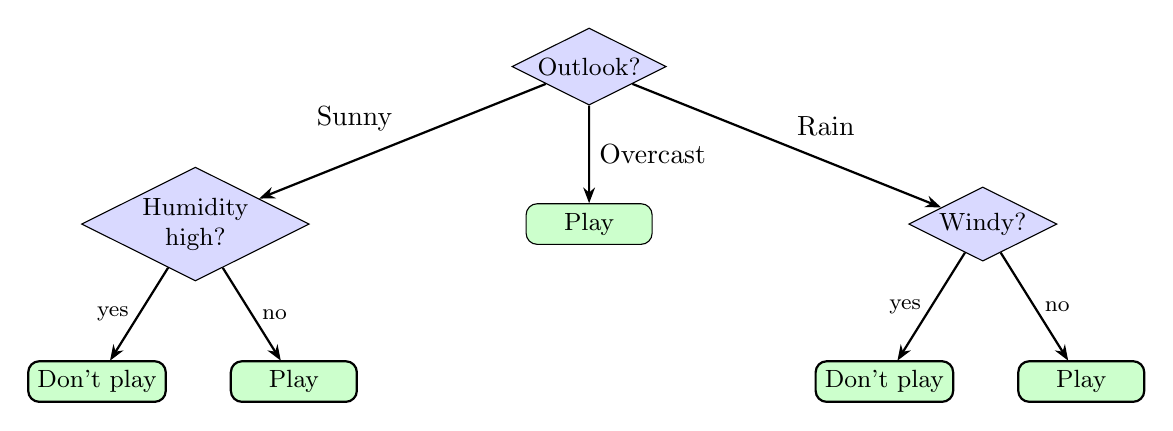
\begin{tikzpicture}[
  level distance=2cm,
  level 1/.style={sibling distance=5cm},
  level 2/.style={sibling distance=2.5cm},
  decision/.style={diamond, draw, fill=blue!15, aspect=2, inner sep=1pt, font=\small},
  leaf/.style={rectangle, rounded corners, draw, fill=green!20, minimum width=1.6cm, font=\small},
  edge from parent/.style={draw, -{Stealth[length=2mm]}, thick},
  every node/.style={align=center}
]
\node[decision] {Outlook?}
  child {node[decision] {Humidity\\high?}
    child {node[leaf] {Don't play} edge from parent node[left, font=\footnotesize] {yes}}
    child {node[leaf] {Play} edge from parent node[right, font=\footnotesize] {no}}
    edge from parent node[above left] {Sunny}
  }
  child {node[leaf] {Play}
    edge from parent node[right] {Overcast}
  }
  child {node[decision] {Windy?}
    child {node[leaf] {Don't play} edge from parent node[left, font=\footnotesize] {yes}}
    child {node[leaf] {Play} edge from parent node[right, font=\footnotesize] {no}}
    edge from parent node[above right] {Rain}
  };
\end{tikzpicture}
\caption{Decision tree for playing tennis.}
\label{fig:decision}
\end{figure}

\end{document}
